\documentclass[conference]{IEEEtran}
%future work: local patch operator
%complexity

\usepackage{subfig}
\usepackage{wrapfig}
\usepackage{amsmath}
\usepackage{url}
\usepackage{pifont}
%\usepackage{times}
\usepackage{rotating}
%\usepackage{balance} 
\usepackage{color, colortbl}
\usepackage{graphicx}
\usepackage{algorithmicx}
\usepackage[running]{lineno}
\usepackage{program}
\usepackage{cite}
\usepackage{alltt}
\usepackage{balance}
\newcommand{\eq}[1]{Equation~\ref{eq:#1}}
\newcommand{\bi}{\begin{itemize}}
	\newcommand{\ei}{\end{itemize}}
\newcommand{\be}{\begin{enumerate}}
	\newcommand{\ee}{\end{enumerate}}
\newcommand{\tion}[1]{\textsection\ref{sec:#1}}
\newcommand{\fig}[1]{Figure~\ref{fig:#1}}
\definecolor{lightgray}{gray}{0.975}
\usepackage{fancyvrb}
\usepackage{stfloats}
\usepackage{multirow}
\usepackage{listings}
\usepackage{amsmath}  
\DeclareMathOperator*{\argmin}{arg\,min} 
\DeclareMathOperator*{\argmax}{arg\,max} 
%\usepackage[usenames]{xcolor}




\usepackage{color}
\newcommand{\colorrule}[1]{\begingroup\color{#1}\hrule\endgroup}

\definecolor{darkgreen}{rgb}{0,0.3,0}

\usepackage[table]{xcolor}
\definecolor{Gray}{rgb}{0.88,1,1}
\definecolor{Gray}{gray}{0.85}
\definecolor{Blue}{RGB}{0,29,193}
\newcommand{\G}{\cellcolor{green}}
\newcommand{\Y}{\cellcolor{yellow}}


\definecolor{MyDarkBlue}{rgb}{0,0.08,0.45} 
\newenvironment{changed}{\par\color{MyDarkBlue}}{\par}

\newcommand{\ADD}[1]{\textcolor{MyDarkBlue}{{\bf #1}}}
\newcommand{\addit}[1]{\begin{changed}\input{#1}\end{changed}}

\usepackage{color}
\usepackage{listings}
\usepackage{setspace}

\definecolor{Gray}{gray}{0.9}
\newcommand{\kw}[1]{\textit{#1}}
\newcommand{\quart}[4]{\begin{picture}(75,6)
	{\color{black}\put(#3,3){\circle*{2.5}}\put(#1,3){\line(1,0){#2}}}\end{picture}}
% New Commands

\definecolor{Code}{rgb}{0,0,0}
\definecolor{Decorators}{rgb}{0.5,0.5,0.5}
\definecolor{Numbers}{rgb}{0.5,0,0}
\definecolor{MatchingBrackets}{rgb}{0.25,0.5,0.5}
\definecolor{Keywords}{rgb}{0,0,1}
\definecolor{self}{rgb}{0,0,0}
\definecolor{Strings}{rgb}{0,0.63,0}
\definecolor{Comments}{rgb}{0,0.63,1}
\definecolor{Comments}{rgb}{0.5,0.5,0.5}
\definecolor{Backquotes}{rgb}{0,0,0}
\definecolor{Classname}{rgb}{0,0,0}
\definecolor{FunctionName}{rgb}{0,0,0}
\definecolor{Operators}{rgb}{0,0,0}
\definecolor{Background}{rgb}{1,1,1}
\title{Actionable = Cluster + Constrast?}

% You can go ahead and credit any number of authors here,
% e.g. one 'row of three' or two rows (consisting of one row of three
% and a second row of one, two or three).
%
% The command \alignauthor (no curly braces needed) should
% precede each author name, affiliation/snail-mail address and
% e-mail address. Additionally, tag each Slope of
% affiliation/address with \affaddr, and tag the
% e-mail address with \email.
%
% 1st. author
\author{Rahul Krishna, Tim Menzies\\
	Computer Science, North Carolina State University, USA\\
	\{i.m.ralk, tim.menzies\}\@gmail.com
	
	% use '\and' if you need 'another row' of author names
	% 4th. author
}


\pagestyle{plain}
\begin{document}
	\maketitle
	\begin{abstract}
		There are many
		algorithms for data {\em classification} such as  C4.5, Naive Bayes, SVM, etc.
		Are these enough for software data analytics? Or should we be supporting
		another kind of reasoning? For example, this paper does not answer 
		``what is'' (i.e. the standard classification problem), but instead  offers advice on ``what to change''.
		Two approaches for learning minimal, yet effective,  changes,  software
		artifacts are explored. Lessons learned are reported.
	\end{abstract}
	\begin{IEEEkeywords}
		Prediction, case-based reasoning, data mining, software engineering.
	\end{IEEEkeywords}
	
	\section{Introduction} 
	How should we handle ``unpopulular'' results
	for data analytics? For example, if a business manager is presented
	with a data mining result that troubles them (e.g. an estimate of
	development time that is distressingly long), what advice
	can we offer them on management actions to {\em change} hat estimate?
	
	This is an important question, and one with much currency in industry.
	In the summer of 2011 and 2012, one of us (Menzies) spent two months
	working on-site at Microsoft Redmond,
	observing data mining analysts.  He
	noted how Microsoft's data scientists
	discussed their data with  business users. 
	One surprising from that study was just how
	little time was spent  
	inspecting  of the output of data miners as compared to another process, which we call {\em peeking}.
	In {\em peeking}, analysts and users spend much time
	inspecting and discuss small samples of either raw or exemplary or synthesized project data.  Further, very little of those discussions were  focused on classification
	(the additional of a labels to some unlabelled data). Rather, much time
	was spent in those meetings discussion {\em what to do next}; i.e. trying
	to determine what could be altered to better improve some business outcome.
	
	That   Microsoft  stufy found two common ``peeking'' methods.
	In {\em data engagement meetings},
	users debated the implications of data
	displayed on a screen. In this way, users
	engaged with the data and with each other by
	monitoring each others' queries and check each others'
	conclusions.
	
	Another data analysis pattern observed
	at Microsoft was  {\em cluster + contrast} in which
	data is  reduced to a few
	clusters. Users are then just shown the delta between those
	clusters. While contrasting, if feature values are
	the same in both clusters, then these were pruned from
	the reports to the user. In this way, very large
	data sets can be shown on one PowerPoint
	slide. Note that {\em cluster+contrast} was a tool that can be usefully employed within
	{\em data engagement meetings}.
	
	
	Cluster+contrast and engagement
	meetings are common practices at Microsoft. Yet  these methods had never been rigorously studied or certified.
	For both those reasons,
	we reflected over those tools to discover and analyze their
	underlying process. The result was HOW: a tool
	that combines (a)~feature selection; (b)~centroid generation from   clusters;
	(c)~contrast methods between centroids.
	While method (a) is widely used (e.g.~\cite{Menzies2010}),
	to the best of our knowledge, this combination of (abc) has not been thoroughly explored before.
	Hence, this paper explores ``peeking''.
	
	\subsection{Digression: Evaluating Changes to a Software Project}
	
Before beginning, we offer three comments on evaluating changes to a project.
Firstly, this paper uses  a prediction system (built by data mining) as the verification
tool for our proposed changes. That is, given a hold out set that is used to learn a predictor,  This means
that the following conclusions are only as certain as the efficacy of the predictor. It could be argued that a better way to assess changes to an organization
would be to implement them in a software project. Indeed, it is true that some organizations have the resources to 
run repeated trials to assess  different treatments.
For example, in one  recent study, Bente et al. report results
were the same  specification   was developed  by four different organizations~\cite{Anda2009}. 
We note that
very few industrial or research groups have access
to the kinds of resources needed for this kind study. Also, given the
diversity of modern software projects, it might be unreasonable to demand that all
proposed changes for all projects are always evaluated by something like the Bente et al. study.

Secondly, an important evaluation criteria for any conclusion made to a business user is that the users can {\em understand} the proposed change. In practice, this means at least
generating {\em succinct} changes. As seen below, not all cluster+contrast methods generate succinct changes.

Thirdly, as a final evaluation criteria, we will demand that the generated recommendations are {\em stable}; i.e. do not widely vary due to minor changes in the data. Hence, in the following, we will add a little randomness to our analysis then report results across 20{\bf XXX} repeated runs. In a result that supports our kind of analysis, we will show that the actions proposed by this analysis are very stable.

	
	\section{How to Cluster}
	Recent results suggest  we are free to select from a wide range of 
	clustering methods.  Ganesan~\cite{div14} explored 
	different clustering methods for SE data using   effort and defect data from
	the PROMISE repository\footnote{http://openscience.us/repo};
	That studied explored
	K-Means, mini-batch-K-Means, DBscan, EM, Ward, and the WHERE algorithm discussed
	below.
	Clusters were assessed via the performance of prediction 
	learned from the clusters by Random Forests (for defect prediction)
	and M5prime or linear regression (for effect estimation).  Ganesan found
	that the details of the clustering method were less important than ensuring that  a large number of clusters were generated.
	
	Accordingly, we select a clustering method that generates $\sqrt{N}$ clusters
	from $N$ examples, that runs fasts, which has shown promise in prior work~\cite{Menzies2013}, and which ignores spurious dimensions (the last item is important since, in our experience, much SE data is ``noisey''; i.e. contains signals not associated with the target variable). For the rest of this article,
	we use  the top-down
	bi-clustering method described in \fig{where} which recursively divides the
	data in two  using a dimension that captures the greatest variability in the data. 
	\begin{figure}[t]
		\small
		~\hrule~
		
		{\bf Step1: Top down clustering using WHERE}
		
		The data is recursively divided in clusters using WHERE as follows:
		\begin{itemize}
			
			\item Find   two   distance cases,  $X,Y$
			by picking any case $W$ at random, then setting $X$ to its most
			distant case, then setting $Y$ to the case most distant from
			$X$
			(this requires only $O(2N)$ comparisons
			of $N$ cases).
			\item Project each case $Z$
			onto a {\tt Slope} that  runs between $X,Y$ using the cosine
			rule. 
			\item Split the data at the median $X$ value of all cases and
			recurses on each half  (stopping when
			one half has less  than $\sqrt{N}$ of the original population).
		\end{itemize}
		~\hrule~
		
		{\bf Step2: Constructing Decision Trees}
		Call each leaf from WHERE a  ``class''. Use an entropy-based
		 decision tree (DT) learner to learn what attributes select for each ``class''. To limit tree size:
		 \bi
		 \item Only use the top $\alpha=33$\%  of the features, as determined by their information gain~\cite{Irani1993}. 
		 \item Only build the trees down to  max depth of $\beta=10$.
		 \item Only build subtrees if it contains at least $N^{\gamma=0.5}$ examples (where $N$ is the size of the training set).
\ei
{\em Score}  DT  leaf nodes  via the mean score of its majority cluster. 
		
		~\hrule~
		
		{\bf Step3: Generating contrast sets}
		\begin{itemize}
		\item Find the {\em current } cluster: take each test instance, run it down to a leaf in the DT tree.  
		\item Find the {\em desired} cluster: 
		\bi
		\item Starting at {\em current}, ascend the tree $lvl\in \{0,1,2...\}$ levels;
		\item Identify {\em sibling} clusters; i.e. leaf clusters that can be reached from level $lvl$ that are not {\em current }
		\item Using the {\em score} defined above, find the {\em better} siblings; i.e. those with a {\em score} less than $\epsilon=0.5$ times the mean score of {\em current}. If none found, then repeat for $lvl += 1$
		\item  Return the {\em closest} better sibling where distance is measured between the mean centroids of that sibling and {\em current}
		\ei
		\item Find the {\em delta}; i.e. the set difference between  conditions in the DT branch to {\em desired} and {\em current}. To find that delta:
		\bi
		\item
		For discrete attributes,  return the value from {\em desired}. 
		\item
		For  numerics, return the numeric difference. 
		\item
		For numerics  into ranges, return a random number selected from the low and high boundaries of the that range.
	\ei
	\ei
		~\hrule~
		\caption{Contrast tree generation: controlled by the parameters
		$\{\alpha, \beta, \gamma, \delta, \epsilon\}$ (set via engineering judgement).}
		\label{fig:contast_trees}
	\end{figure}
	
	\section{How to Contrast}
	Once we have  clusters, the next task is to offer business users lessons learned from comparing different clusters.
		Once methods for doing so are the {\em contrast trees} and the {\em instance-based}
		methods discussed below.
	
		\subsection{ Contrast Trees}

Contrast trees were first developed by Lekkalapudi and Menzies as a method
for explaining reasoning within multi-objective optimization~\cite{nva14}. This paper is the first
application of contrast trees to defect prediction.

	Contrast trees start by clustering data to find clusters $C_1,C_2,...$.
	Next, using those clusters as class labels, we execute a decision tree algorithm to find what attributes select for different clusters. After that, to learn recommendations for a business user, we determine (1) what {\em current} cluster are you in?; (2) what {\em desired} cluster do you want to move to?; (3) what is the delta between those clusters? To answer the last question, we report the delta in the branches of the decision tree that lead to {\em current} and {\em desired}.  For full details, see \fig{contast-trees}.
	
	%Contrast trees are decision trees that can be used to learn decision rules from a large data set. The use of decision trees for this purpose makes it easy to visualize the data and also makes interpretation of the recommended policies fairly straight forward. In addition to this, contrast tree generate ranges of decisions that allow for better feasibility.
 
 

	\begin{figure}[t]
		{\footnotesize  \begin{tabular}{{llrrc}}
				\arrayrulecolor[gray]{.90}
				\rowcolor[gray]{.95} \textbf{Rank} & \textbf{Treatment} & \textbf{Median} & \textbf{IQR} & \\
				1 &     Ant (Tree) &    0.67  &  0.41 & \quart{0}{39}{37}{69} \\
				1 &     Ant (HOW) &    0.7  &  0.13 & \quart{33}{13}{40}{69} \\
				1 &   Jedit(HOW) &    0.72  &  0.25 & \quart{25}{24}{42}{69} \\
				1 &   Jedit (Tree) &    0.75  &  0.13 & \quart{37}{12}{43}{66} \\
				\hline \end{tabular}}
		
		\caption{Results comparing the performance scores on sample projects from the Jurezcko data sets.}
		\label{res}

	\end{figure}
	
	
	\begin{figure*}[!t] 
		\begin{minipage}{0.5\linewidth}
			\subfloat[Tree Learner]{
				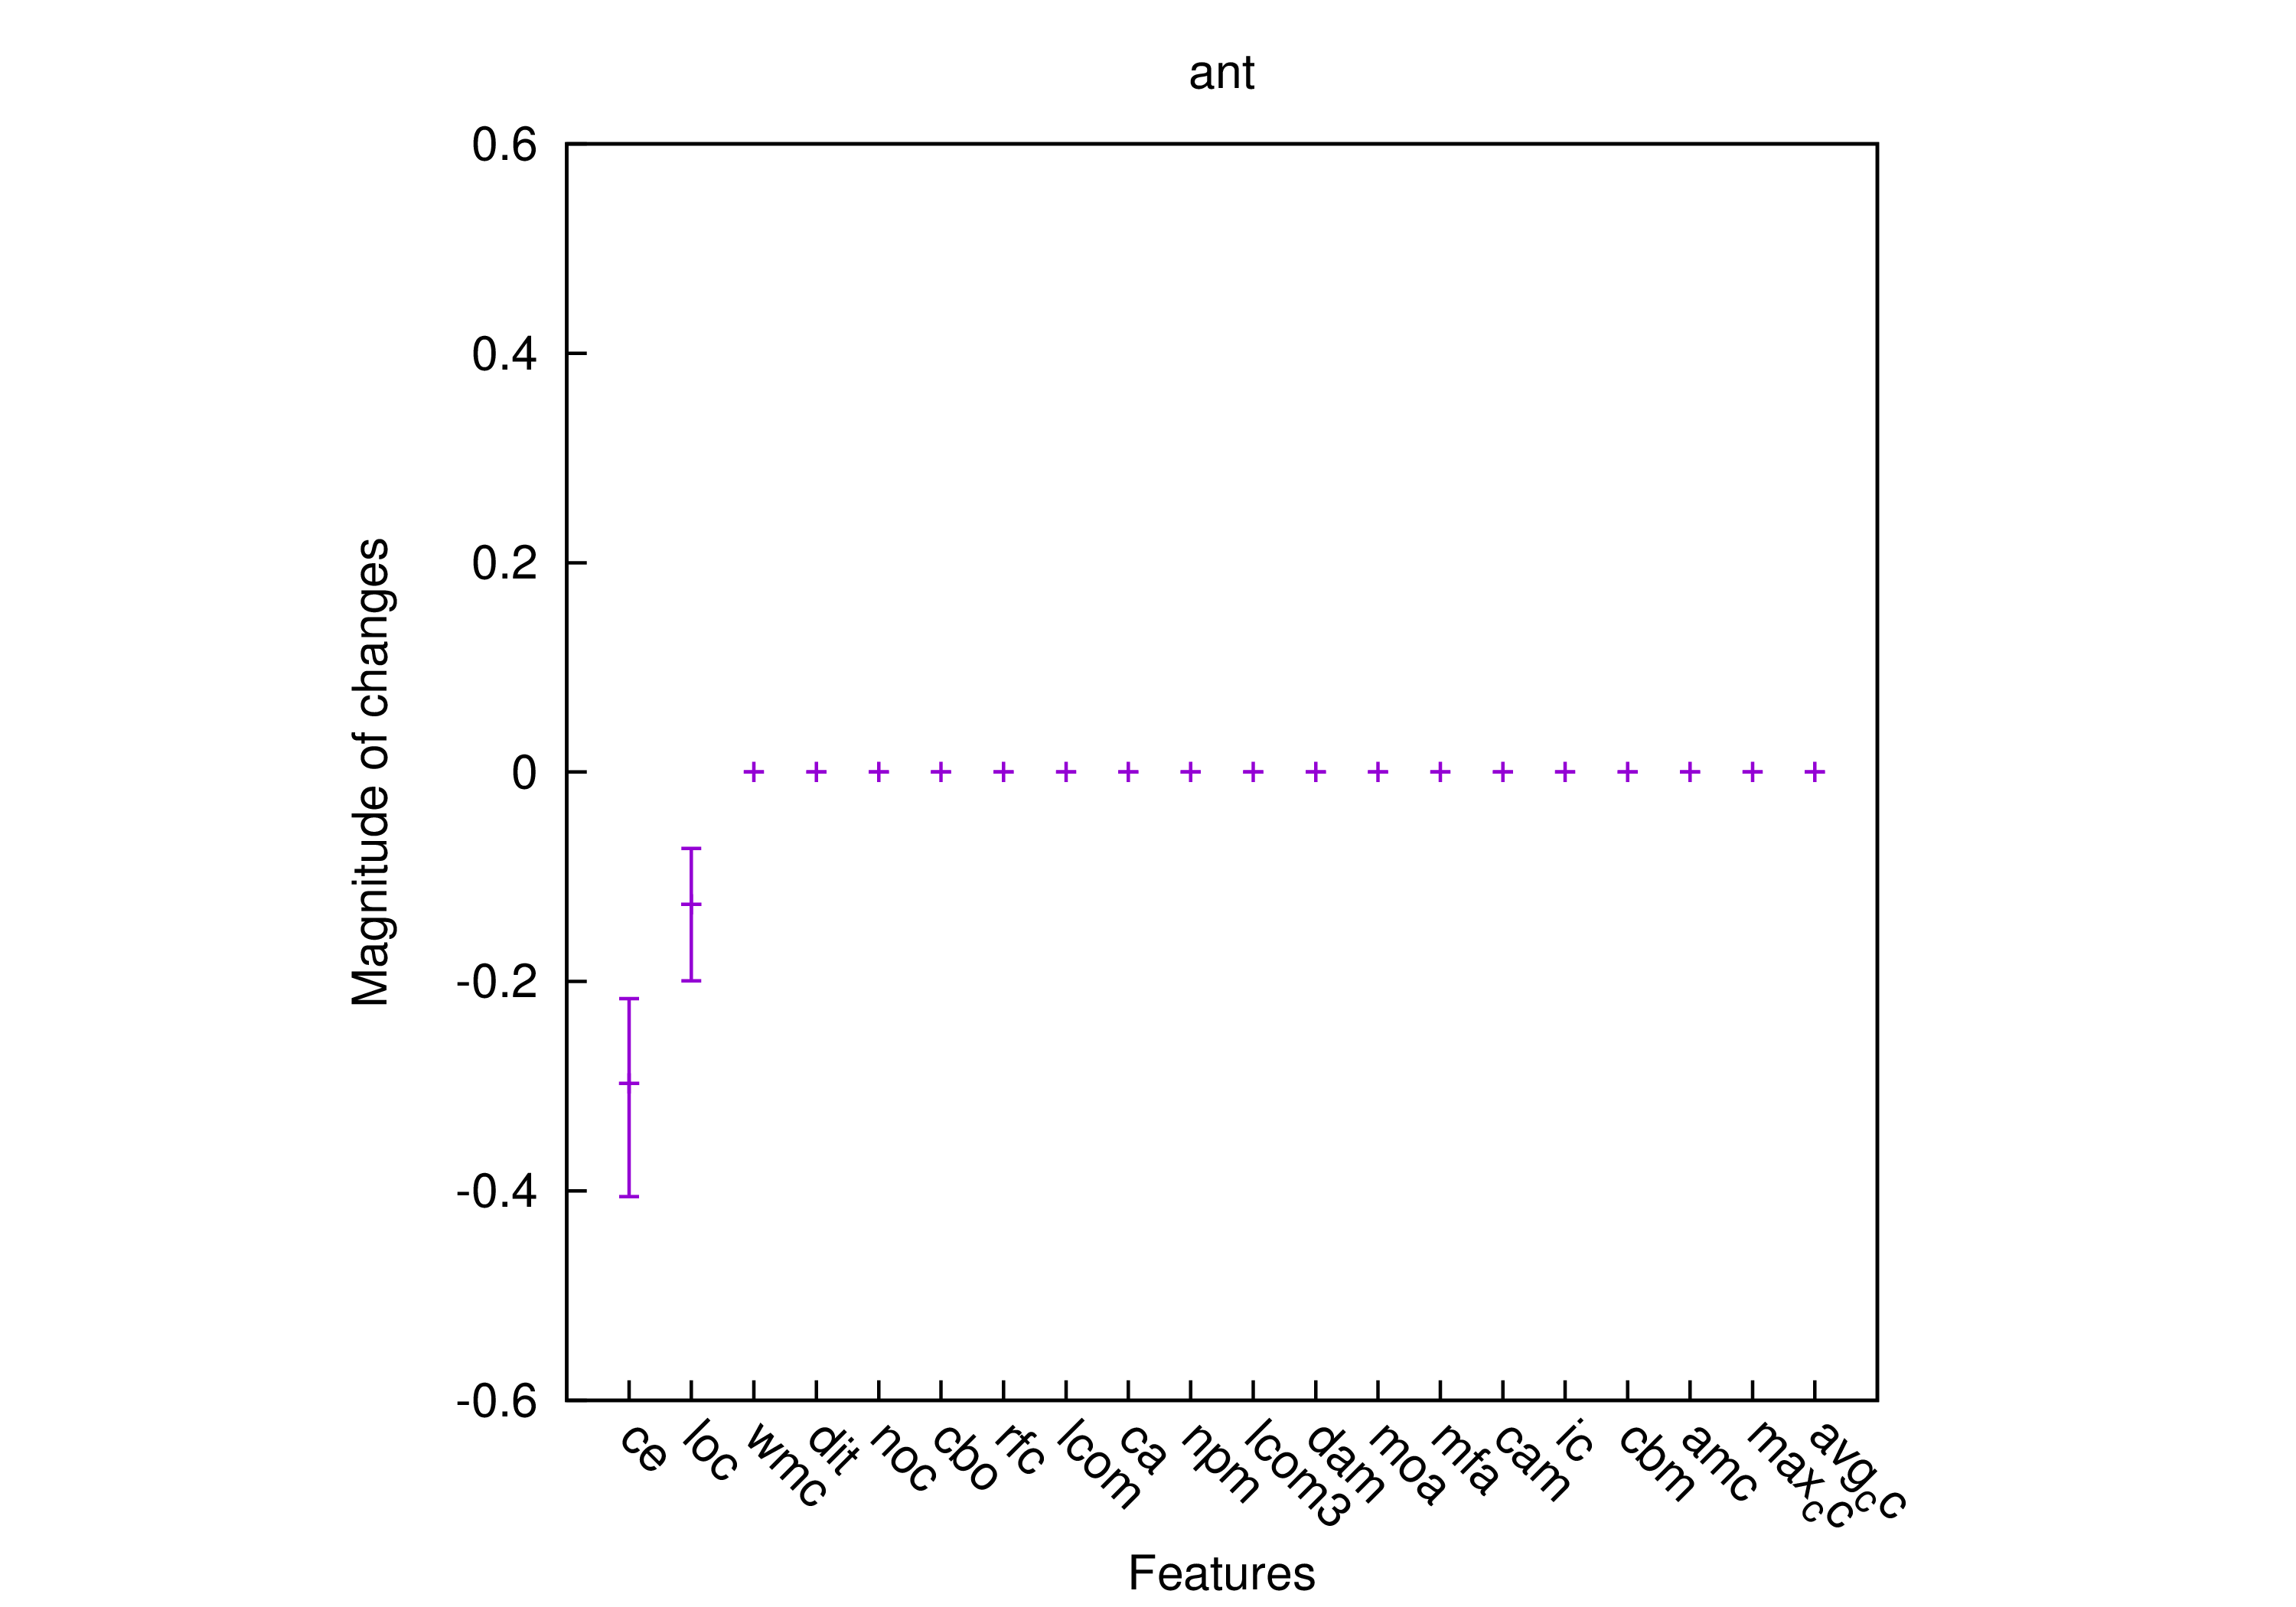
\includegraphics[width=\linewidth]{ant1.png}
				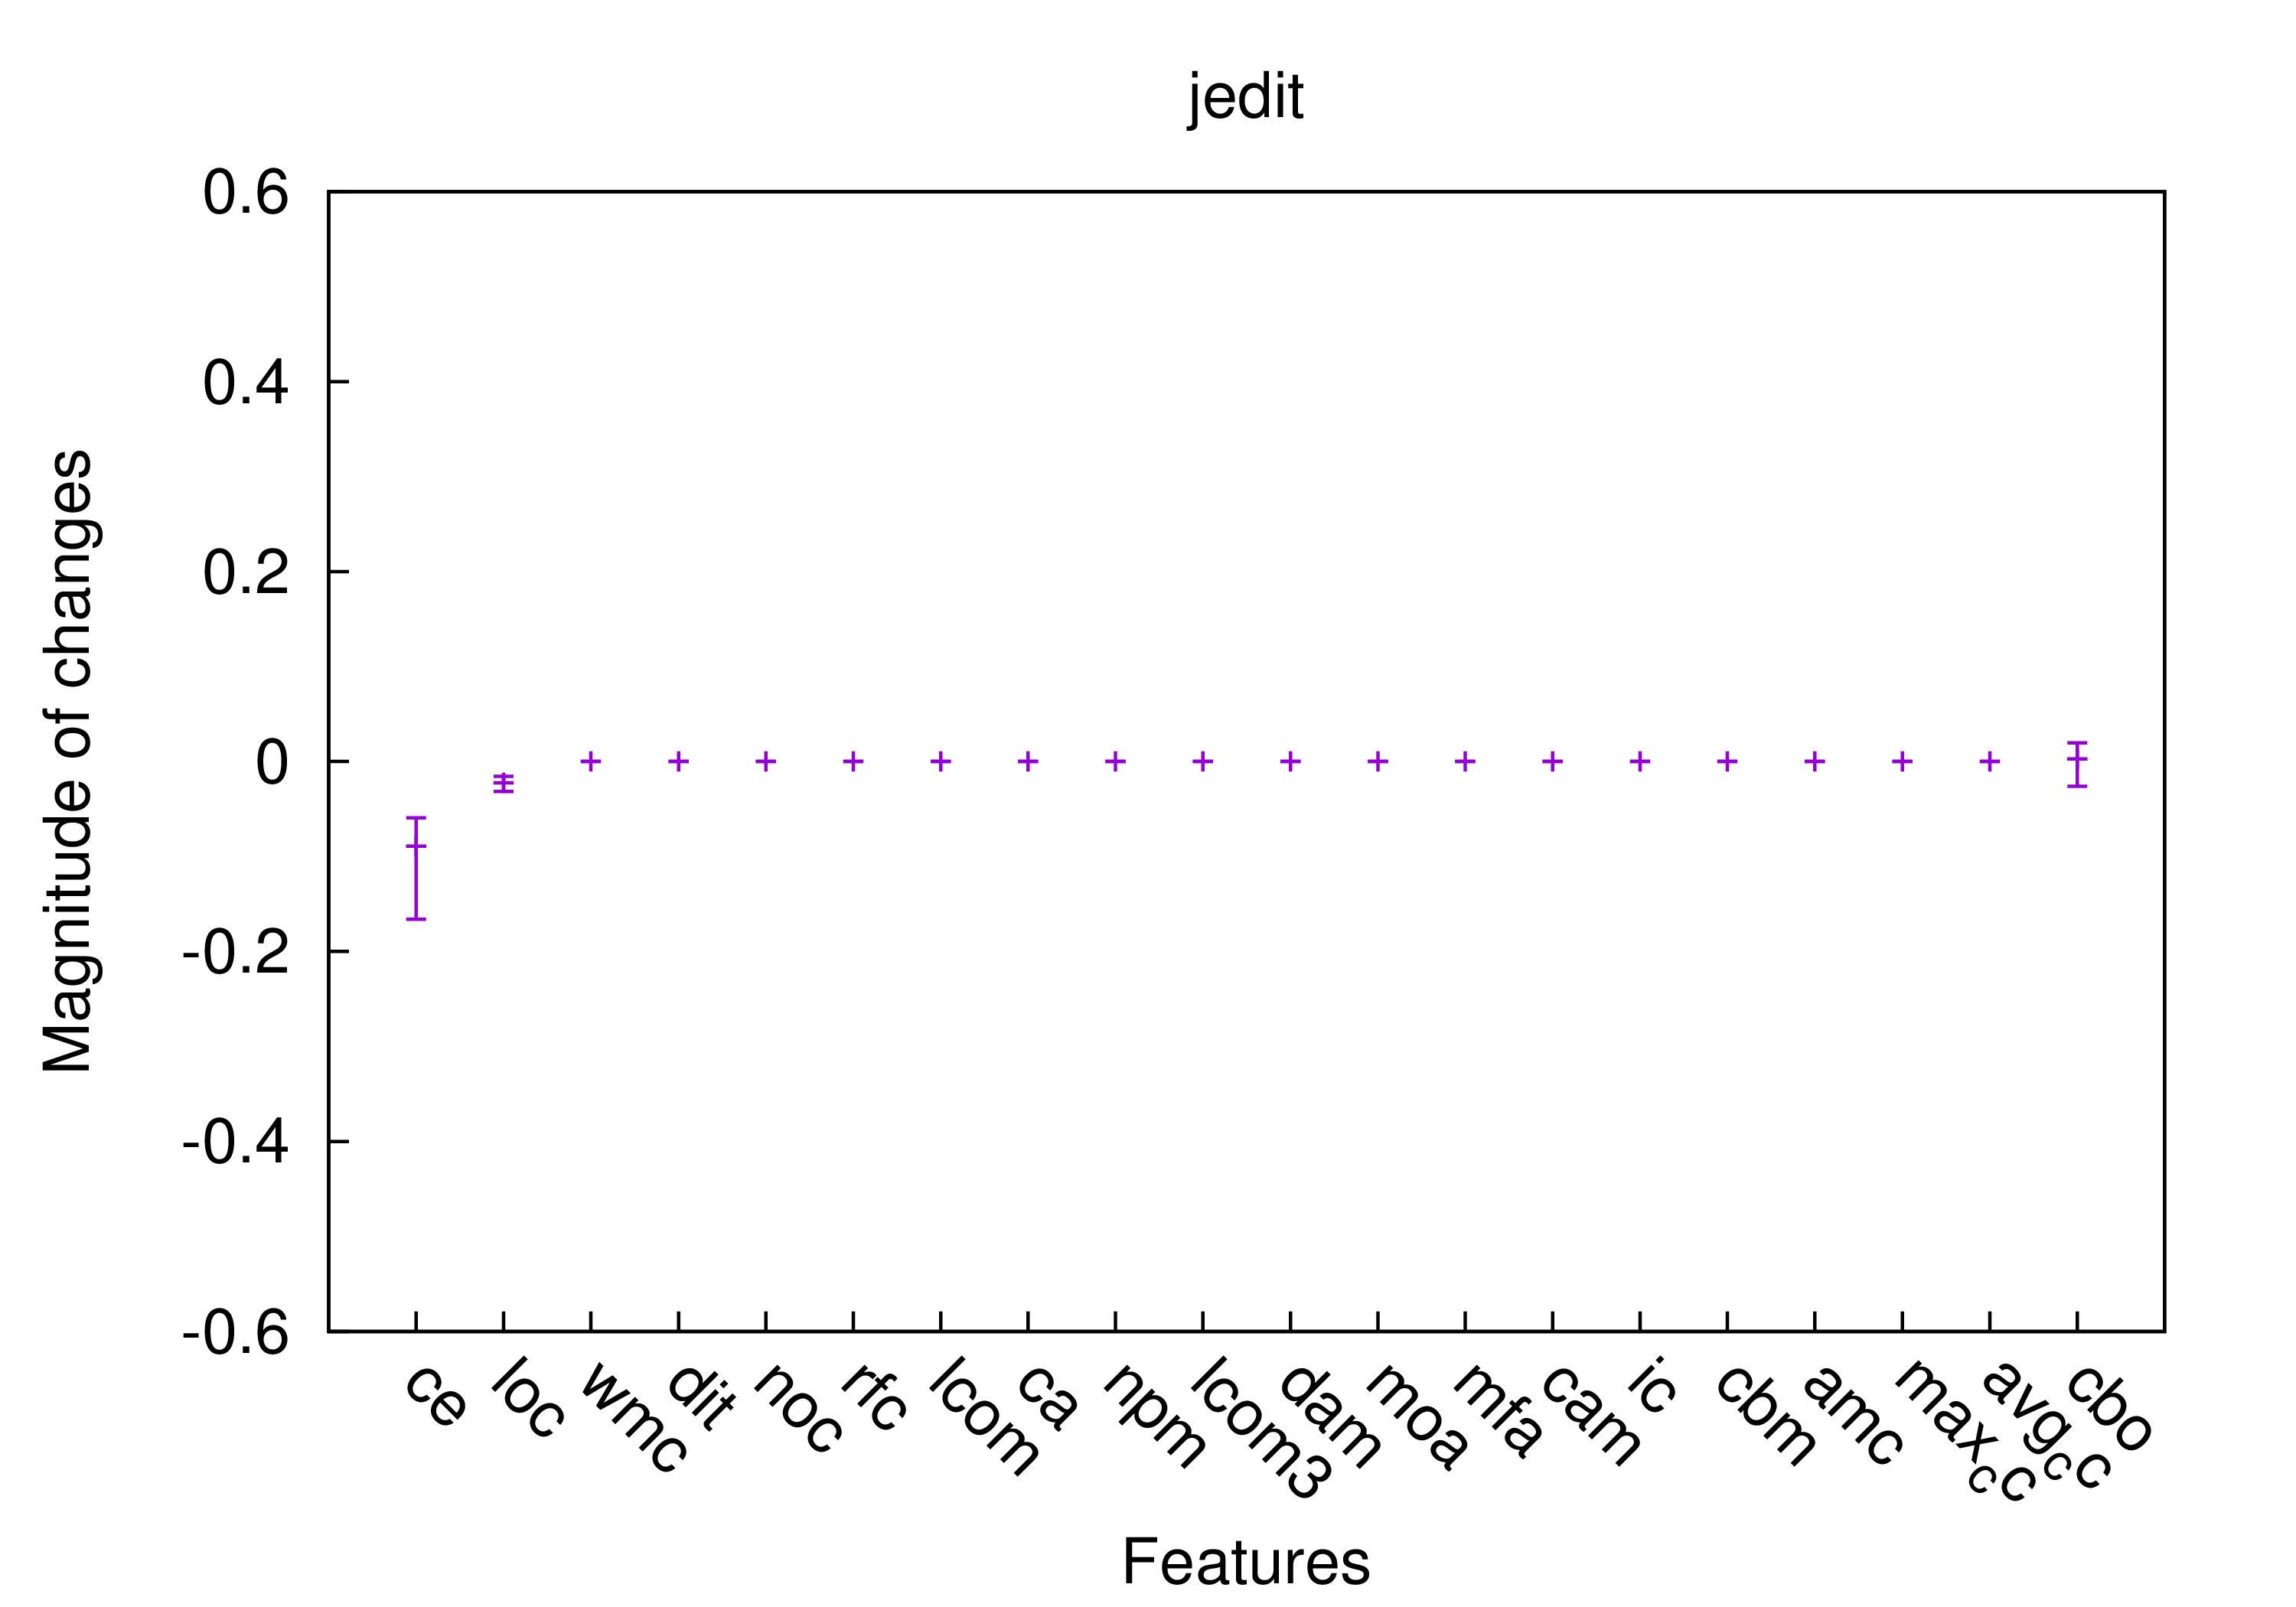
\includegraphics[width=\linewidth]{jedit1.png}}\\
			\subfloat[HOW]{			
				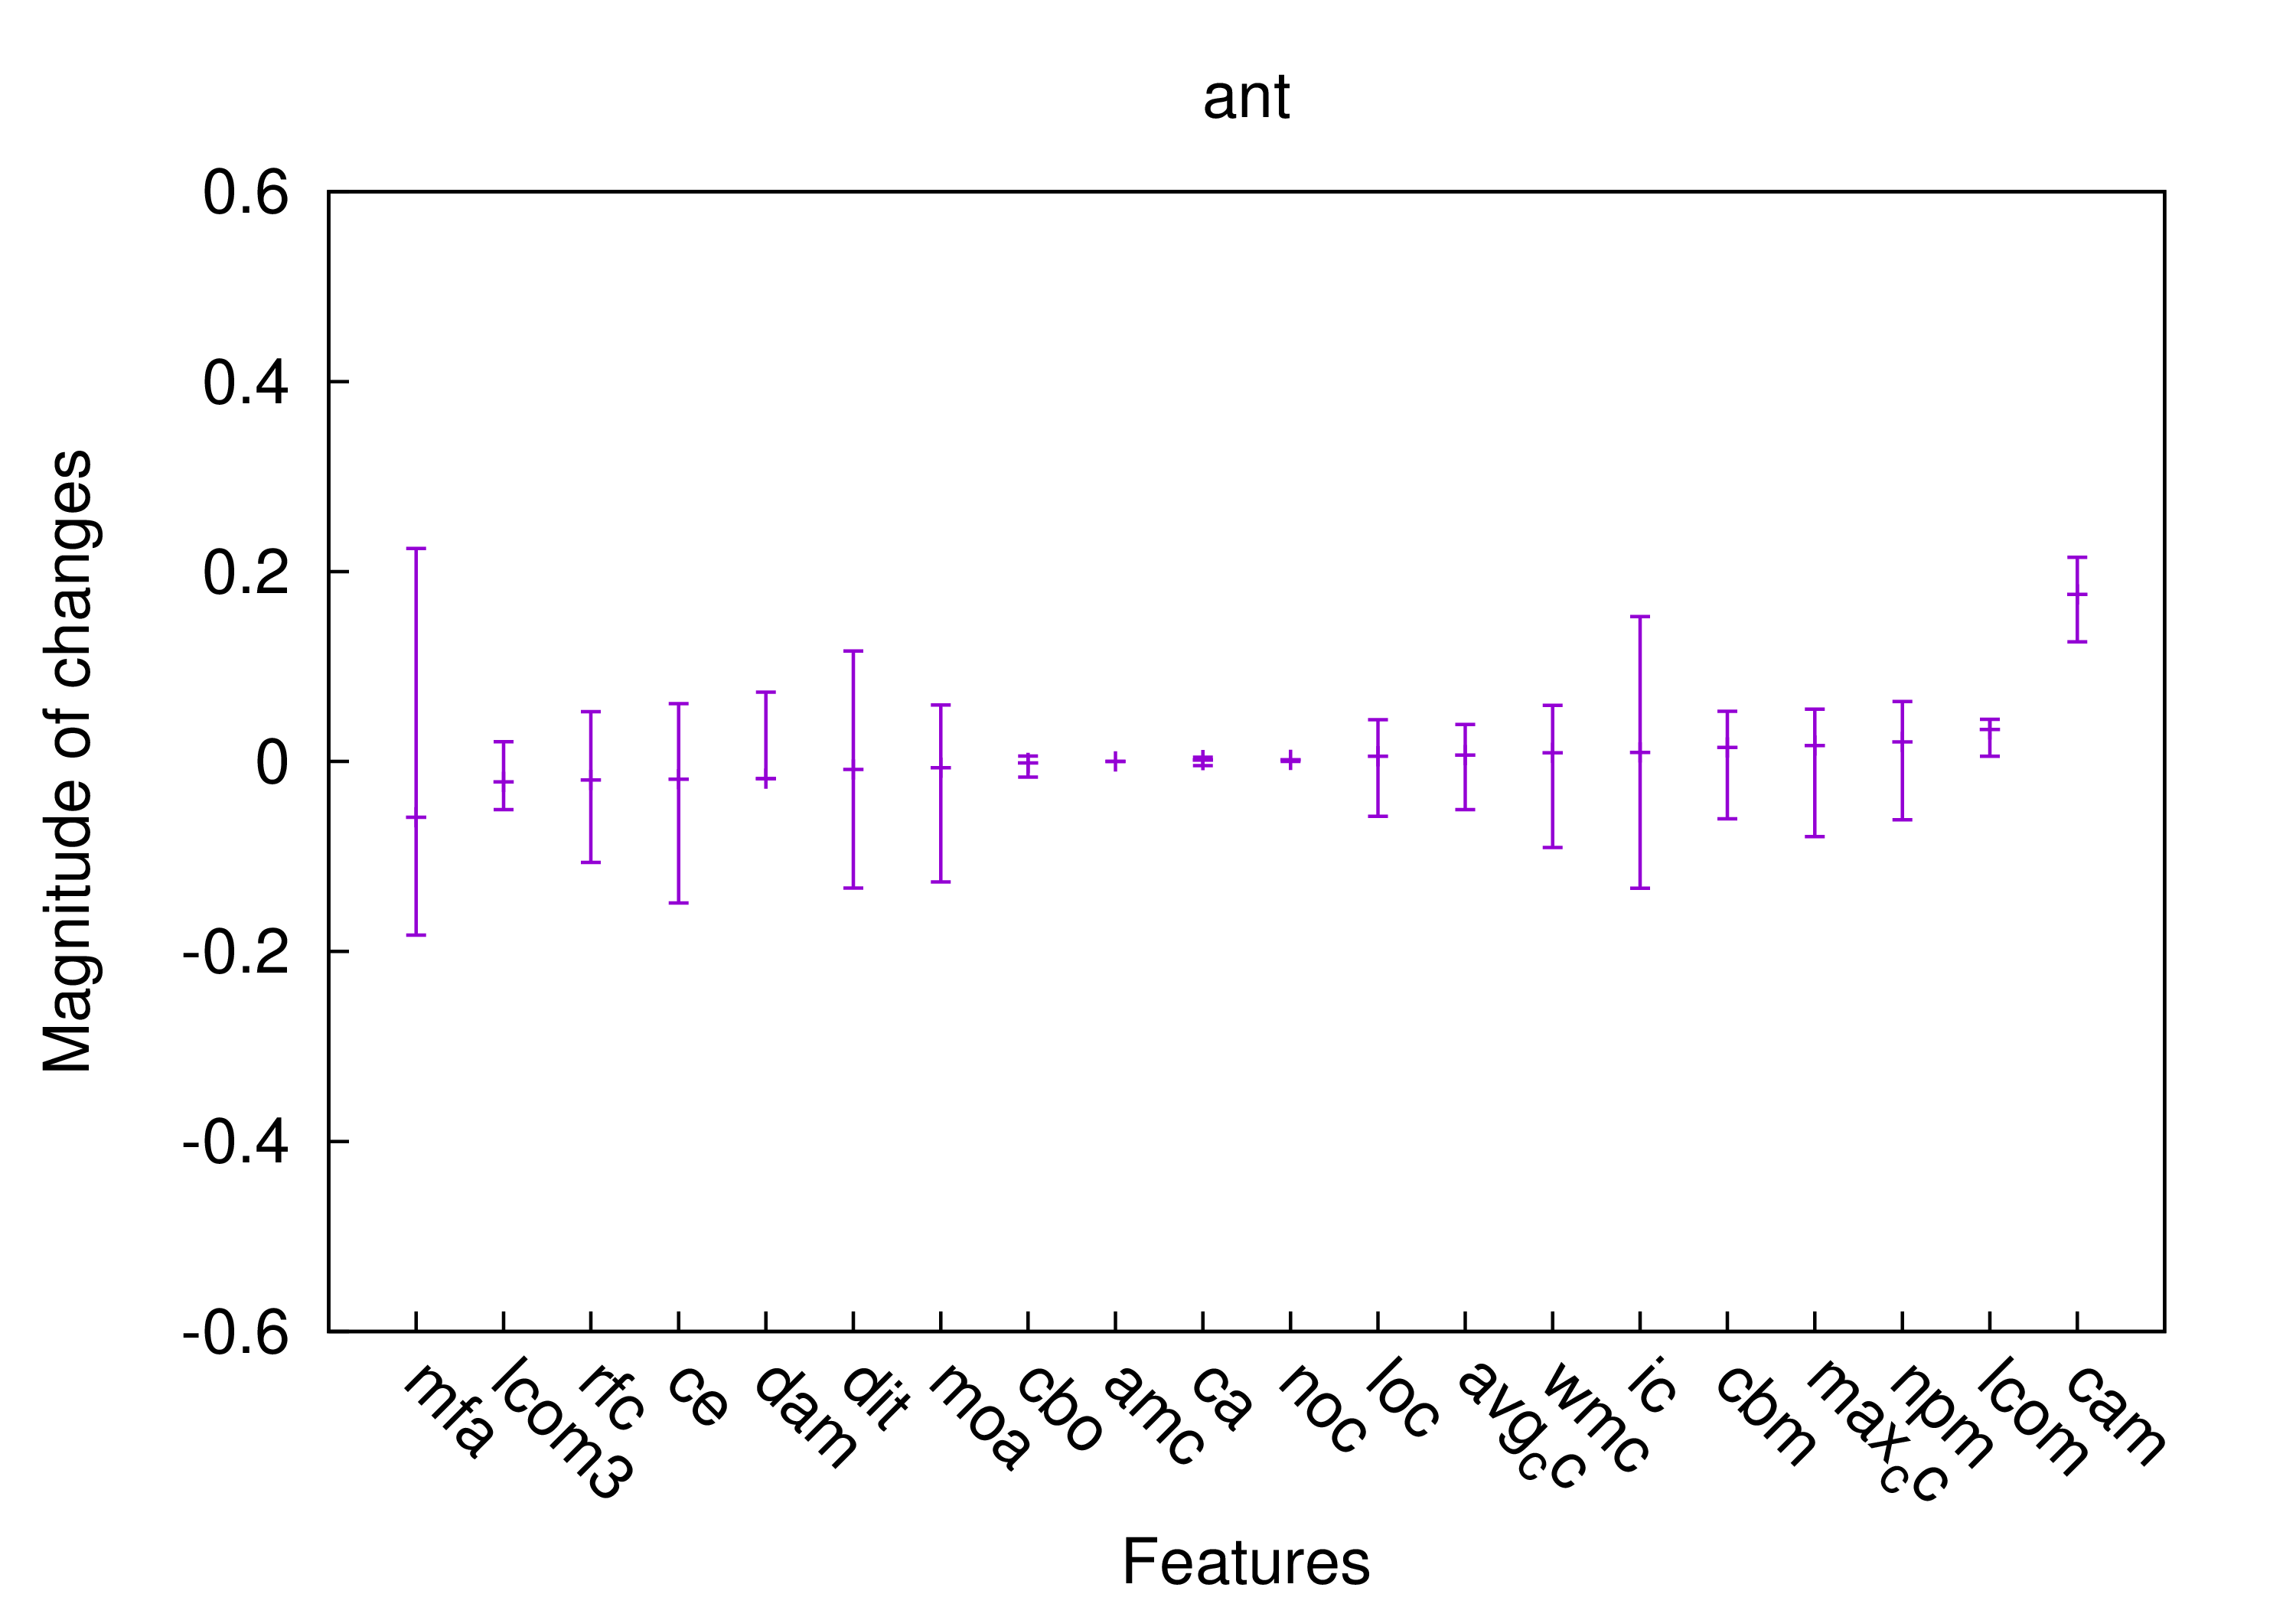
\includegraphics[width=\linewidth]{ant2.png}
				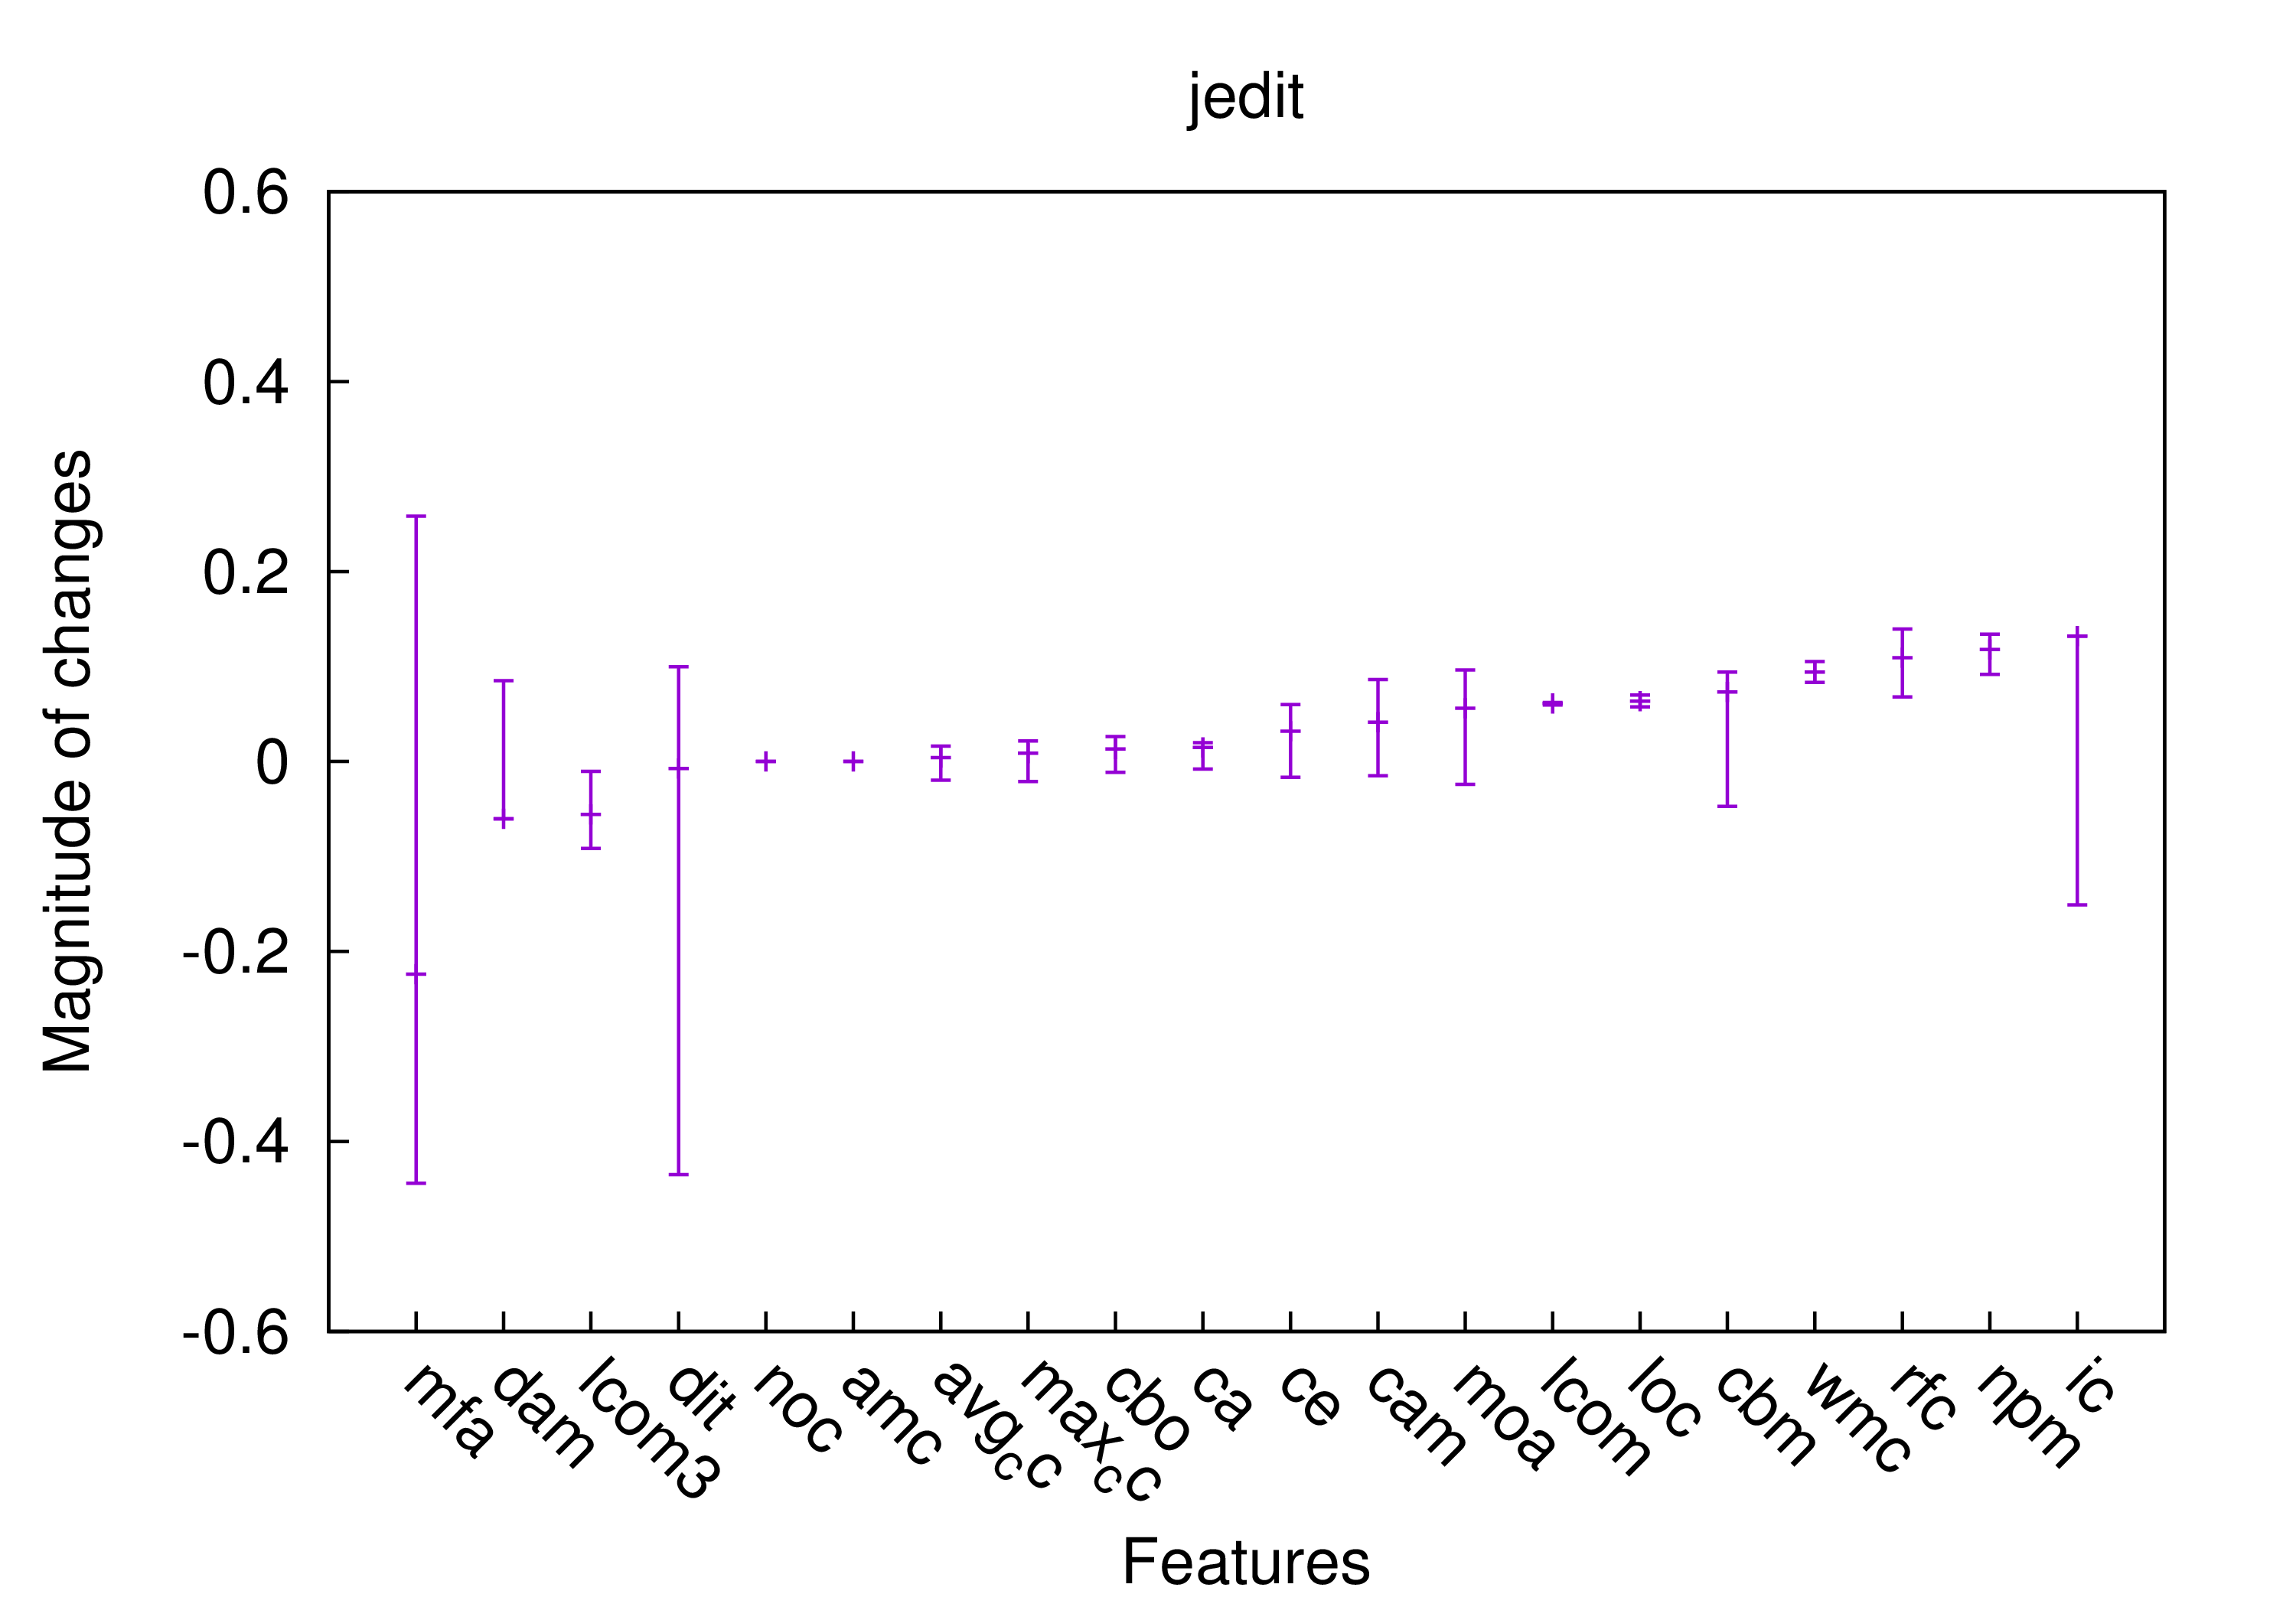
\includegraphics[width=\linewidth]{jedit2.png}}
		\end{minipage}
		\caption{Performance Comparision}
		\label{deltas}
	\end{figure*}
	

As with any tree structure, the size and depth of the contrast tree has a profound impact on it performance. Our initial motivation was that the trees could serve as a medium for experts to identify and explore solution spaces that were local to the problem. The size of the decision tree, if too large, jeopardizes the readability of the solutions by increasing the complexity. We have therefore made efforts to reduce the size of the tree using  a pruning method that prunes away irrelevant branches that do not contribute better solutions (see step2 of \fig{contast-trees}). The smaller trees are much easier to understand.



	\subsection{Instance-based Contrasts}
	Contrast tree represents the next generation of our efforts to use contrast set learners for planning and case based reasoning. All the other methods were {\em instance-based reasoners}
	\bi
	\teim  W2 was an instance-based planner that reflected over the delta of raw attributes \cite{6600685}. However, it frequently suffered from an optimization failure. When its plans were applied, performance improved in only $\tfrac{1}{3}$rd of test cases. 
	
	Generation two of our work resulted in the development of contrast trees. As briefly discussed above, it uses a recursive clustering algorithm followed by summarizing these recursive divisions into a tree structure. The initial results with contrast tree was very encouraging. As a continuation of our contrast tree work, we built HOW~\cite{HOW} as a simpler approach that was to provide a baseline result, above which contrast tree was meant to do better. 
	
	HOW is very different to other CBR systems in that it explores the {\em gradient between pairs of nearest clusters}. In other words, the classic CBR methods, including Contrast Trees, explore {\em points} while
HOW explores the slope {\em between} points. Experimentation with HOW provided results that were in fact comparable to Contrast Trees. 
	
	\section{Experiments}
	\subsection{Data}
	For our initial experimentation, we studied two sample projects from the Jureczko object-oriented static code data sets~\cite{jureczko10}: Ant, Camel, Ivy, Jedit,   Log4, Lucene, Poi, Synapse, Velocity, Xalan, Xerces \footnote{Available from the object-oriented defects section of the PROMISE respository openscience.us/repo/defect/ck.}. The data is a collection of 20 OO measures and a the Boolean dependent attribute (whether a defect is reported to a post-release bug-tracking system). For our study, we picked two projects, Ant and Jedit, that best exemplified the performance of Contrast Tree. 
	\subsection{Assessment}
	In this study we wish to demonstrate Contrast Trees' ability to suggest meaningful changes in order to reduce defects while obtaining baseline results using a simpler algorithm. All our results have been presented as ratios of the number of defects after applying the recommended changes to the original number of defects (so numbers less than 1.0 indicate improvements). A Scott-Knott procedure was used to test for statistically significant differences in the results.
The Scott-Knott procedure recommended by Mittas \& Angelis in their 2013
IEEE TSE paper~\cite{mittas13}. The samples for the Scott-Knott were obtained by repeating our experiments at least 20 times (the value of 20 was chosen as the minimum use sample size via the central limit theorem).
	
	In addition to this, we also explored the magnitude of changes that are being recommended. Specifically, we wanted to study if the changes too small or too large to be practically implemented. We measure these changes as a difference between the original attribute and the changed attributes, normalized to lie between $\pm1$. 
	\subsection{Results}
	The results of figure \ref{res} shows that in both of our
 data sets, Contrast Trees' results are ranked exactly the same as the results seen
 with HOW. That is, statistically, there are no differences between the two techniques. 
 
 However, looking at what changes each of the techniques suggest, the differences are patent. As seen in figure \ref{deltas}, the plans obtained using Contrast Trees require that the changes be made to significantly fewer attributes while those with HOW require that some changes be made to all the attributes of the data. In addition to this, below are some of key advantages presented by Contrast Trees over other algorithms:
	
	\begin{itemize}
		\item They allow the user to exert a fine grain control over the parameters that needs to be changed, while providing a way to visualize the recommended changes.
		\item The changes suggested by the contrast sets are inherently local in nature, making the changes practical and potentially easy to implement.
		\item The contrast tress require a worst case time complexity of $O(n)$, which is a function in linear time.
	\end{itemize}

Therefore, preliminary experimentation suggest that Contrast  Trees  are  an excellent tool to efficiently identify the key features that require changes, and also  to  obtain  a  quantitative  measure  as  to  how much change needs to be made.

	\subsection{Discussion}

 
	\section{Future Work}
	Now, we strongly recommend HOW over contrast tree (and W2) since, as shown by the following results, HOW’s plans never lead to performance getting worse. Also, when HOW did improve the expected values of the performance, those performance improvements were an order of magnitude larger than those seen with contrast tree. 
\bibliographystyle{plain}
\bibliography{hownot}
\end{document}